
\begin{frame}{Kinase regulation model}
\label{sec:Heinrich}

\begin{columns}
\begin{column}{0.5\textwidth}


% Protein phosphorylation is a ubiquitous means of regulating protein activity controlled by protein kinases and phosphatases. Kinase cascades allows a signal from outside the cell to propagate into the nucleus via phosphorylation events as modelled by Heinrich~et~al.~\cite{Heinrich2002kinase}.

% The signal can be described as a single activated receptor sending a signal that decays with rate~$\lambda^{(\text{Receptor})}$, and where each protein kinase has a single protein kinase input~(\autoref{fig:kinase_cascade}). The change in phosphorylation of a kinase $i$ is modelled as follows:
Kinase cascade, each protein with single input~\cite{Heinrich2002kinase}
\begin{subequations}
\label{eq:kinase_cascade}
\begin{align}
\dv{\phi_i}{t} &=
    \tilde{w}_i \phi_{i-1} \tilde{\phi}_i - \lambda_i^{(\text{Phos})} \phi_i
\\
    &=
    w_i \phi_{i-1} \left(1 - \frac{\phi_i}{p_i}\right) - \lambda_i^{(\text{Phos})} \phi_i
\\
p_i &= \phi_i + \tilde{\phi}_i
\,,\,
w_i = \tilde{w}_i p_i
\end{align}
\end{subequations}

% Here, $\phi_i$ is the amount of phosphorylated protein $i$ and $\tilde{\phi}_i$ is the unphosphorylated amount. $w_i$ is the kinase rate of phosphorylation by phosphorylated protein $i-1$ on unphosphorylated protein $i$, and $\lambda_i^\text{Phos}$ is the decay rate of the phosphate group on protein $i$, which is controlled by the reaction of all the phosphatases in the cell with protein $i$. 
% It is assumed that a phosphorylation event is always an unphosphorylated kinase being phosphorylated by another kinase which itself is phosphorylated.

% The regulation generalizes to include the possibility of multiple inputs of regulation onto each protein kinase, which can be written with vector notations~(\autoref{eq:kinase_general}).

Generalized, any protein can affect any protein
\begin{subequations}
\label{eq:kinase_general}
\begin{align}
\dv{\phi_i}{t} &=
    \left( \sum_j w_{ij} \phi_j \right) \left(1 - \frac{\phi_i}{p_i}\right) - \lambda_i^{(\text{Phos})} \phi_i
\\
\label{eq:matrix_kinase}
\dv{\boldsymbol{\phi}}{t} &= (W \boldsymbol{\phi}) \left(1 - \frac{\boldsymbol{\phi}}{\boldsymbol{p}}\right) - \Lambda_\text{Phos} \boldsymbol{\phi}
\end{align}
\end{subequations}

% Here $w_{ij}$ is the regulation effect from node $j$ to $i$, which is a positive value. The division in~\autoref{eq:matrix_kinase} is an elementwise division.


\end{column}
% \begin{column}{0.5\textwidth}
% \begin{figure}
% \begin{minipage}[c]{0.42\textwidth}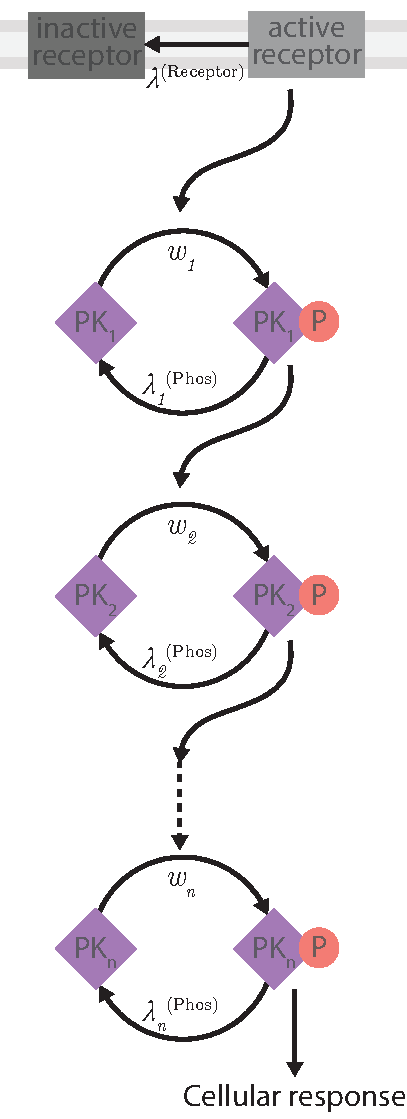
\includegraphics[width=\textwidth]{theory/fig/kinase_cascade.pdf}\end{minipage}
% \begin{minipage}[t]{0.54\textwidth}\caption{\textbf{Kinase cascade with single inputs.} A protein kinase cascade transmitting a signal from a cell membrane receptor.}\end{minipage}
% \label{fig:kinase_cascade}
% \end{figure}
% \end{column}

\begin{column}{0.5\textwidth}
\begin{figure}
\begin{minipage}[t]{0.4\textwidth}
\caption{\textbf{Kinase cascade with single inputs.} Transmitting signal from a membrane receptor.}
\end{minipage}
\begin{minipage}[c]{0.37\textwidth}
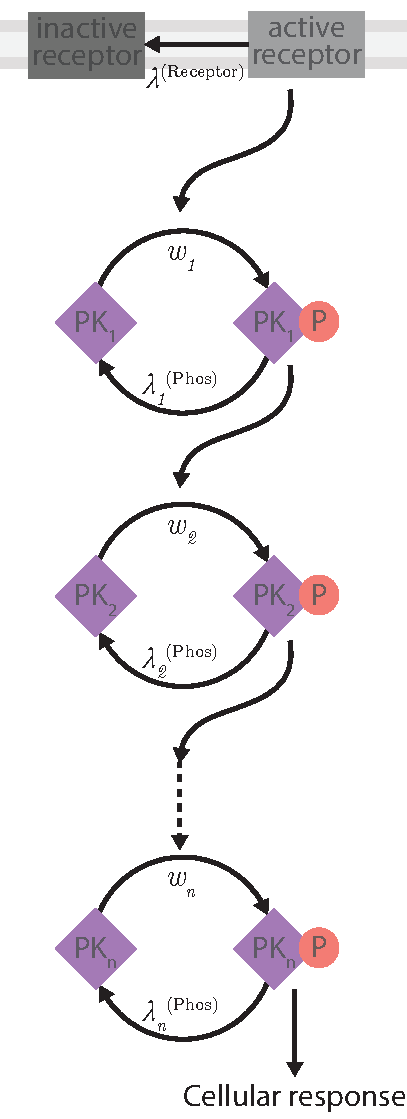
\includegraphics[width=\textwidth]{theory/fig/kinase_cascade.pdf}
\end{minipage}
\label{fig:kinase_cascade}
\end{figure}
\end{column}
\end{columns}
\end{frame}


